\documentclass[a4paper, 12pt]{article}

\usepackage[utf8]{inputenc}
\usepackage{geometry}
\usepackage{polski}
\usepackage{graphicx} 
\usepackage{float} 
\usepackage{etoolbox,refcount}
\usepackage{multicol}
\usepackage{fancyhdr}
\usepackage{listings}
\usepackage{amsmath}
\usepackage{tabularx}

\pdfsuppresswarningpagegroup=1
\newgeometry{left=2.5cm, right=2.5cm, bottom=2.5cm, top=2.5cm}

\author{Adrian Jałoszewski\\ Automatyka i Robotyka, Grupa 2}
\title{Baza danych infrastruktury telekomunikacyjnej}
\date{}

\begin{document}
    \maketitle
    \section{Identyfikacja dziedziny projektu}
        Projekt dotyczy zaprojektowania bazy danych do zarządzania infrastrukturą
        telekomunikacyjną. Zawiera ona informacje na temat tego jakie metryki są 
        liczone i zbierane dla zarządzanych urządzeń, ich lokalizację, danych oraz 
        producentów. W bazie danych znajdują się również awarie wraz z informacjami
        o tym kto je naprawił i gdzie pracownik ten pracuje. 
        \\ \\
        W tej bazie danych można wyróżnić cztery części:
        \begin{itemize}
            \item[--] Przechowywanie wyznaczonych metryk
            \item[--] Przechowywanie informacji o urządzeniu
            \item[--] Przechowywanie informacji o lokalizacji urządzenia i
                pracowników.
            \item[--] Przechowywanie informacji o naprawach dokonywanych na
                urządzeniach.
        \end{itemize}
        Wyznaczone metryki mogą być używane do tworzenia KPIów lub do określania
        zachowania SLA. Przykładami takich metryk są np. liczba gubionych pakietów
        lub downtime w danym okresie czasu.
        \\ \\
        Posiadanie informacji na temat lokalizacji geograficznej urządeń pozwala
        na efektywne zatrudnianie pracowników tak aby byli jak najbliżej urządzeń.
        \\ \\
        Posiadanie informacji na temat używanych produktów i producentów pozwala
        na lepsze planowanie przyszłych inwestycji (produkty jednego producenta mogą 
        współpracować lepiej z jego innymi produktami).
        \\ \\
        Informacje o naprawach pozwalają określić awaryjność danego urządzenia oraz 
        pozwalają określać tendencję do psucia się danego produktu oraz monitorować
        naprawy sprzętu (czas od awarii do naprawy i trwanie naprawy).
    \section{Typowe zapytania użytkowanika}
        \begin{enumerate}
            \item Który producent produkuje najbardziej awaryjny sprzęt.
            \item Który model rutera jest najbardziej awaryjny.
            \item Który pracownik w ciągu swojej kariery naprawił najwięcej
                sprzętu firmy Cisco.
            \item Liczba pracowników w mieście w którym nastąpiła największa
                liczba awarii.
            \item Dziesięć najgorszych urządzeń w kategoriach downtime.
            \item Dziesięć urządzeń najczęściej gubiących pakiety w Berlinie.
            \item Ile urządzeń znajduje się w Kopenhadze.
            \item W którym miesiącu miało miejsce najwięcej awarii.
            \item Jak dużo urządzeń firmy Juniper naprawili pracownicy z Krakowa
                poza Krakowa. 
            \item Ile awarii wynikało z błędnej konfiguracji.
            \item Liczba pakietów zgubionych w Niemczech w 2017 roku.
        \end{enumerate}
    \section{Założenia i ograniczenia}
        \subsection{Miasto}
            Miasto musi mieć nazwę oraz być w kraju, który posiada nazwę.
        \subsection{Miejsce pracy}
            Miejsce pracy musi się znajdować w mieście, mieć nazwę oraz adres.
        \subsection{Pracownik}
            Pracownik musi mieć miejsce pracy, imię, nazwisko oraz może mieć
            email. Pracownika nie można usunąć z bazy danych jeżeli dokonywał
            naprawy jakiegoś urządzenia -- jest to konieczne do zachowania 
            informacji o nim w raportach.
        \subsection{Producent}
            Producent sprzętu musi mieć email w przypadku konieczności kontaktu,
            stronę internetową oraz nazwę firmy. Producent nie może zostać usunięty
            z bazy danych dopóki wykorzystywane są jego produkty.
        \subsection{Produkt}
            Produkt musi mieć nazwę oraz określony typ. Typ jest dowolny, 
            ponieważ w pewnej chwili firma zarządzająca siecią może chcieć 
            dodać nowy rodzaj nadajnika GSM, który mógł nie zostać uwzględniony.
            Nie można usunąć informacji o produkcie dopóki są wykorzystywane 
            urządzenia tego typu.
        \subsection{Urządzenie}
            Urządzenie musi mieć identyfikator wewnętrzny do używania z innymi
            systemami. Urządzenie musi być jednym z produktów w bazie danych
            oraz posiadać lokalizację.
        \subsection{Metryka i wartości metryki}
            Metryka musi mieć nazwę oraz jednostkę. W oddzielnej tabeli są 
            przechowywane wartości zebrane dla danej metryki wraz z chwilami
            czasu w UTC, których dotyczą. W przypadku usunięcia metryki lub
            urządzenia dla którego liczona jest metryka usuwane są wszystkie
            próbki.
            \\ \\
            Metryki są zbierane z dokładnością co do sekundy.
        \subsection{Awaria}    
            Awaria ma dwa stany -- przed dokonaniem naprawy oraz po dokonaniu
            naprawy. W przypadku gdy naprawa nie miała jeszcze miejsca mogą być 
            problemy z określeniem następujących pól (dlatego ich uzupełnienie 
            jest wymagane w chwili zakończenia naprawy):
            \begin{itemize}
                \item[--] koszt
                \item[--] opis
                \item[--] przyczyna
                \item[--] serwisowanie na miejscu
            \end{itemize}
            Serwisowanie kończy się w chwili kiedy jest ustalana data zakończenia.
            W tym przypadku są sprawdzane wszystkie parametry pod względem
            kompletności.
            \\ \\
            Czas zakończenia naprawy dodatkowo musi być albo nieustawiony albo 
            większy od czasu rozpoczęcia naprawy. Czas rozpoczęcia naprawy musi
            być albo nieustawiony albo większy od czasu zgłoszenia awarii. Czas
            wystąpienia awarii musi być ustawiony.
            \\ \\
            Awarie są monitorowane z dokładnością co do dnia.
    \section{Diagram ER} 
        \begin{figure}[H]
            \centering
            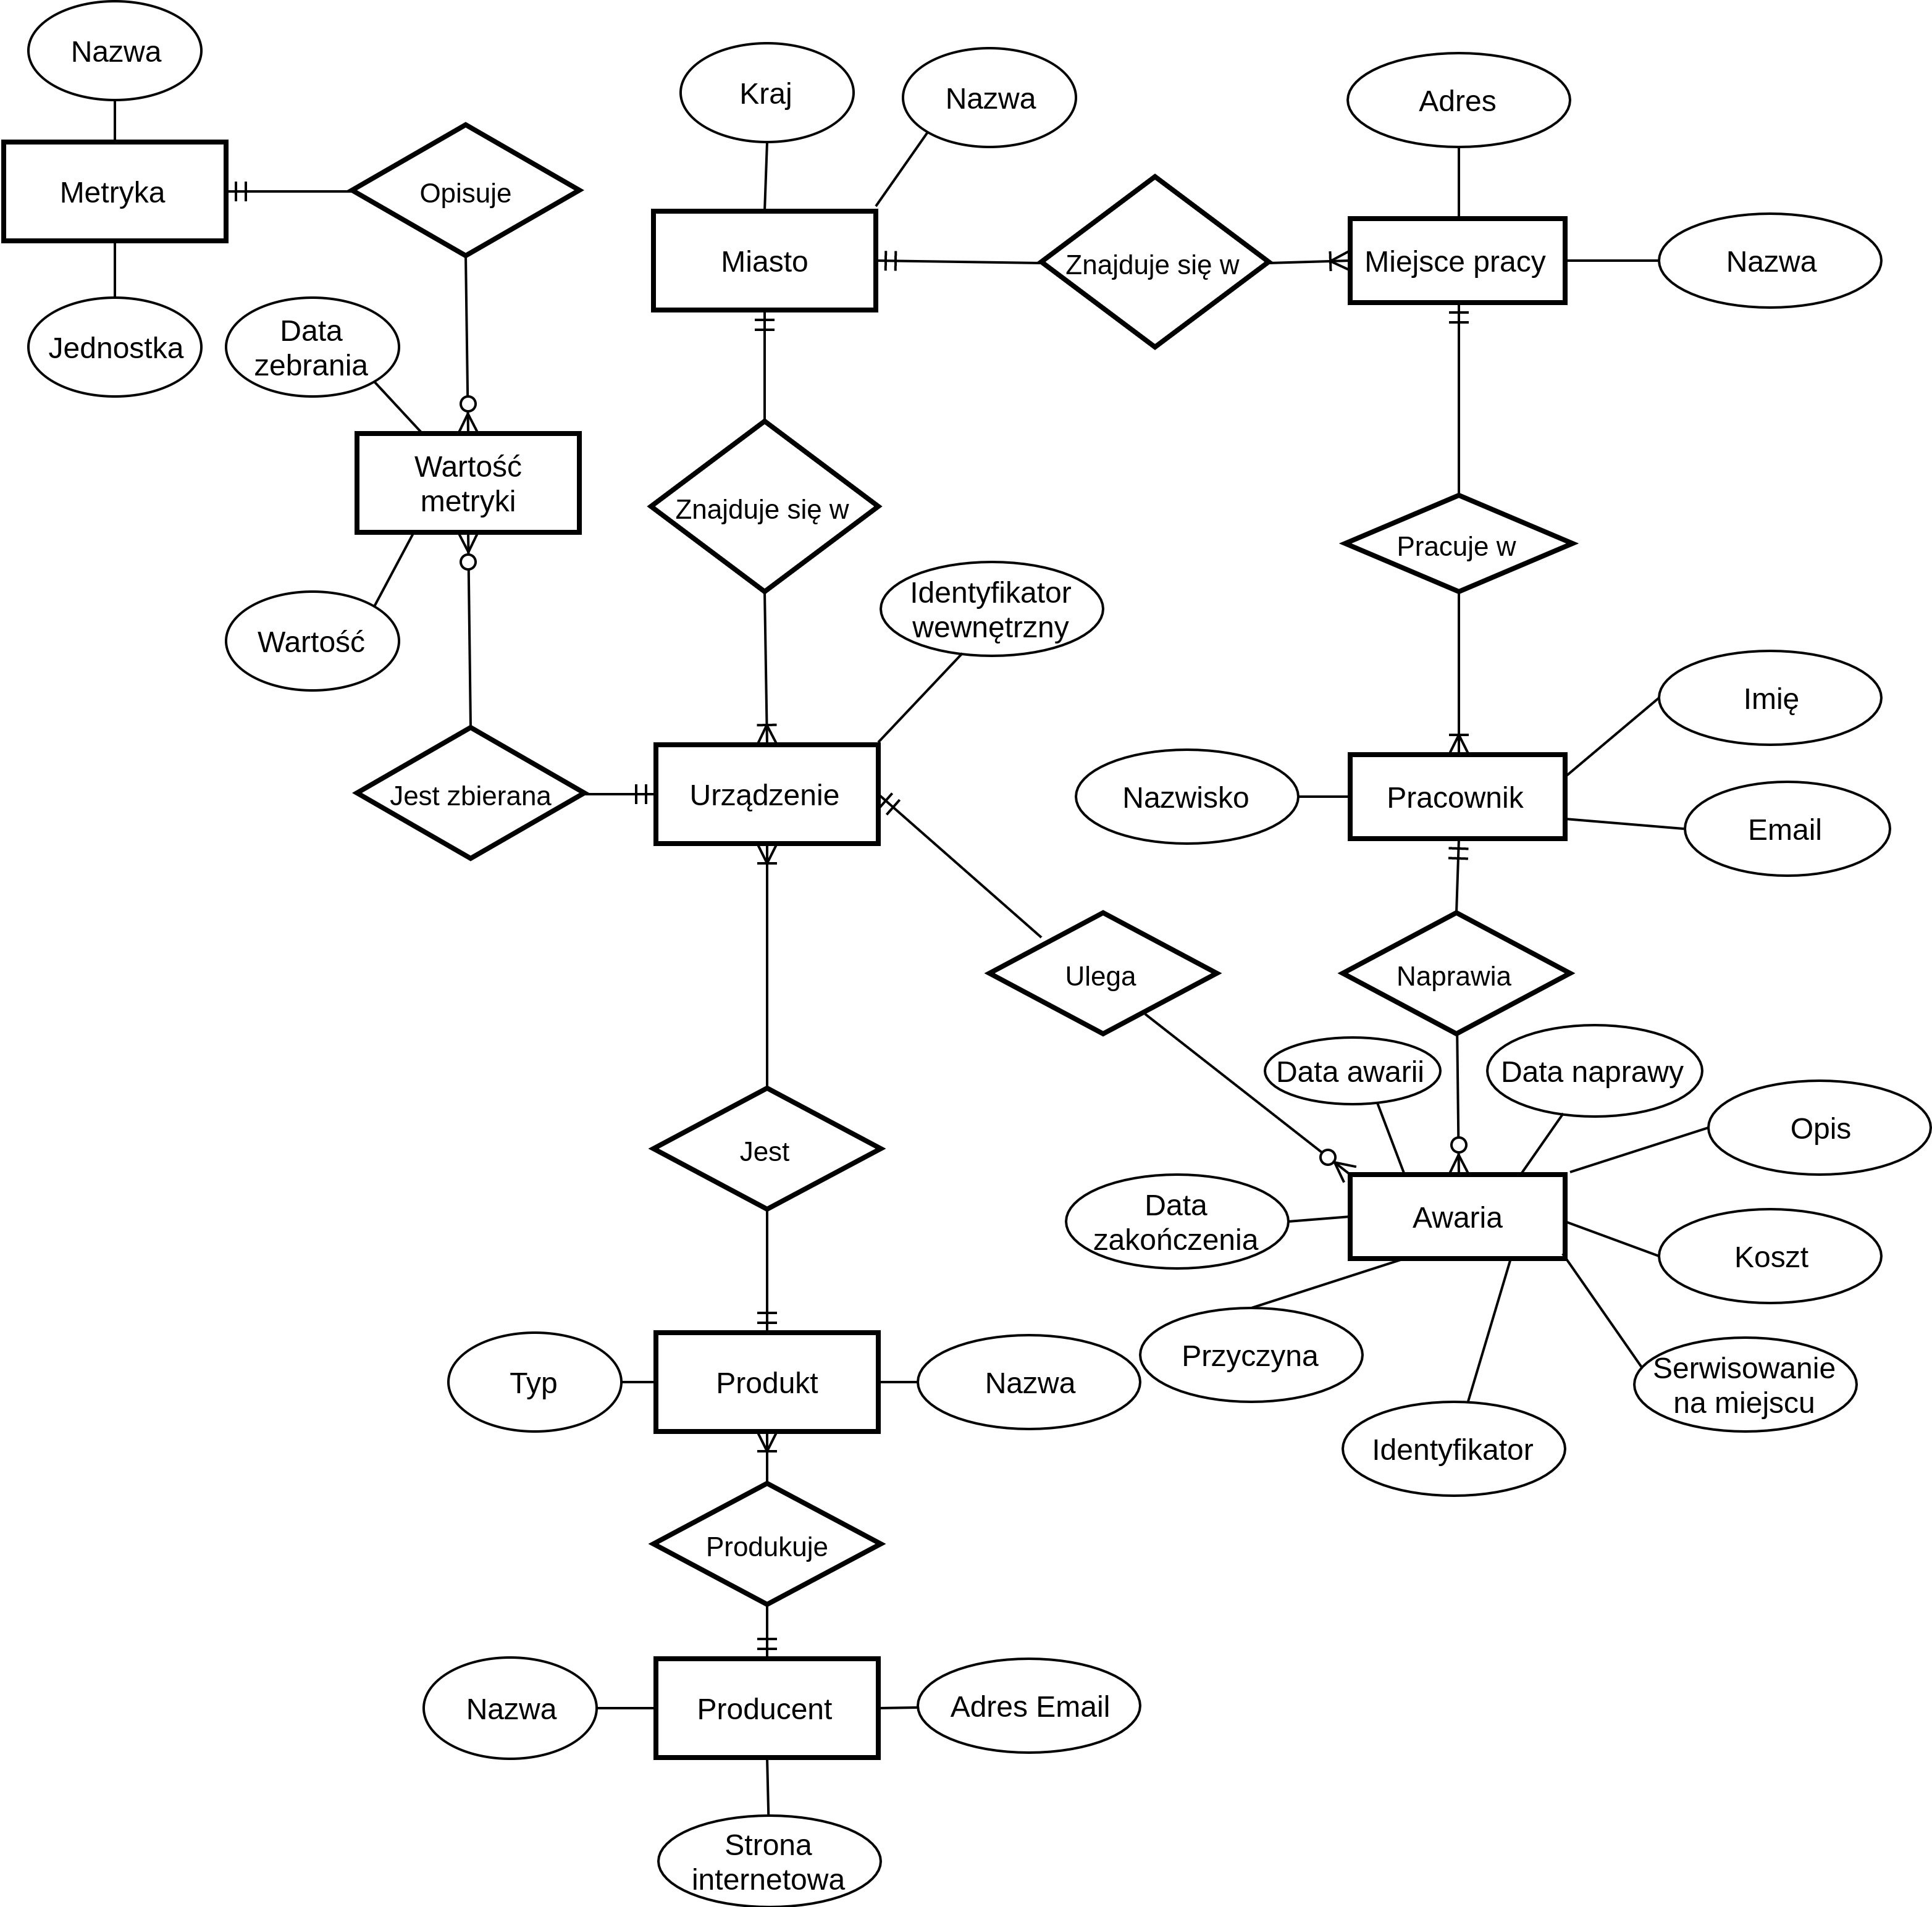
\includegraphics[width=\textwidth]{er.png}
        \end{figure} 
\end{document}
